%% =============================================================================
%% presentation/slides.tex — Beamer deck for 5-min bachelor's defence
%% Topic: VPN application with 2FA (WireGuard-based)
%% Author: Валюх А.А.  |  Supervisor: Бойко Ю.В.  |  Kyiv 2026
%%
%% Engine: XeLaTeX (2 passes)
%% Spec: storyboard.md R2 + thesis preamble.tex font mirror
%% 7 main frames + appendix backup frames (R1–R6)
%% =============================================================================

\documentclass[aspectratio=43,14pt]{beamer}

%% ─── Language & Fonts (mirror thesis preamble.tex) ───────────────────────────
\usepackage{fontspec}
\usepackage{polyglossia}
\setmainlanguage{ukrainian}
\setotherlanguage{english}
\setmainfont{Times New Roman}
\setsansfont{Arial}
\setmonofont[Script=Default,Scale=MatchLowercase]{Courier New}
\newfontfamily\cyrillicfonttt[Scale=MatchLowercase]{Courier New}

%% ─── Graphics & TikZ ──────────────────────────────────────────────────────────
\usepackage{graphicx}
\graphicspath{{../images/}}           % for R5 func-*.png screenshots
\usepackage{tikz}
\usetikzlibrary{arrows.meta,positioning,calc,backgrounds,fit,shapes.geometric}

%% ─── Figure scaling helper (max width/height, aspect-ratio preserved) ─────────
\usepackage{adjustbox}

%% ─── Tables ───────────────────────────────────────────────────────────────────
\usepackage{booktabs}
\usepackage{array}
\usepackage{tabularx}

%% ─── Misc utility ─────────────────────────────────────────────────────────────
\usepackage{xcolor}
%% QR code for R7 backup frame (XeLaTeX-compatible; pure TikZ rendering)
\usepackage[nolinks]{qrcode}

%% ─── Beamer theme: default, strip ALL ornament ───────────────────────────────
\usetheme{default}
\usecolortheme{default}
\usefonttheme{professionalfonts}   % honour fontspec setup, no Beamer substitution

%% Remove every navigational / decorative element
\setbeamertemplate{navigation symbols}{}
%% Minimal footline: frame number only, bottom-right, grey, discreet.
%% clGrey is a \definecolor name — use \textcolor, not \usebeamercolor.
%% [plain] frames (title) suppress this automatically; also wrapped explicitly below.
\setbeamertemplate{footline}{%
  \hfill\textcolor{clGrey}{\scriptsize\insertframenumber}\hspace{1.2em}%
  \vspace{0.8em}%
}
\setbeamertemplate{headline}{}
\setbeamertemplate{background}{}
\setbeamertemplate{sidebar right}{}
\setbeamertemplate{sidebar left}{}

%% Minimal frametitle: 1–2 word grey label, NO bar, NO border
\setbeamertemplate{frametitle}{%
  \vspace*{0.30em}%
  {\usebeamerfont{frametitle}\usebeamercolor[fg]{frametitle}%
   \insertframetitle\strut}%
  \vspace*{-0.25em}%
}

%% ─── Colour palette (must match figures/styles.tex exactly) ─────────────────
\definecolor{clInk}{HTML}{1A1A1A}
\definecolor{clAccent}{HTML}{1F3A5F}
\definecolor{clGrey}{HTML}{7A7A7A}
\definecolor{clBg}{HTML}{FFFFFF}

%% Apply palette to Beamer elements
\setbeamercolor{normal text}{fg=clInk, bg=clBg}
\setbeamercolor{frametitle}{fg=clGrey, bg=clBg}
\setbeamercolor{structure}{fg=clAccent}
\setbeamercolor{alerted text}{fg=clAccent}
\setbeamercolor{itemize item}{fg=clAccent}
\setbeamercolor{enumerate item}{fg=clAccent}
\setbeamercolor{block title}{fg=clAccent, bg=clBg}
\setbeamercolor{block body}{fg=clInk, bg=clBg}
\usebeamercolor{normal text}

%% Frametitle font: small sans-serif — label only, no banner
\setbeamerfont{frametitle}{size=\small, series=\mdseries, family=\sffamily}

%% ─── Shared TikZ styles (shared interface with diagram-dev) ──────────────────
%% presentation/figures/styles.tex
%% Shared palette and TikZ node styles — loaded once in slides.tex preamble.
%% Every fig-XXX.tex file assumes this has been \input{} before it.
%% Canonical source: storyboard.md §«Палітра та кодування».
%%
%% ENCODING CONTRACT (projector-safe, colourblind-safe):
%%   cmark / xmark  → redundant by GLYPH SHAPE; colour reinforces
%%   add / remove   → redundant by LINE STYLE (solid / dashed); colour reinforces
%%   present / gone → redundant by FILL (solid / hollow); colour reinforces
%% No red or green used anywhere.
%%
%% NOTE: NO blank lines inside \tikzset{} — blank lines create \par which
%% pgfkeys cannot handle.  Use %% comment lines as separators instead.
\usepackage{pifont}    %% \ding{} for shape-encoded checkmark / cross
%%
%% ── Palette (3-colour: ink + accent + grey) ─────────────────────────────────
\definecolor{clInk}{HTML}{1A1A1A}     % near-black  — text, lines, "present" nodes
\definecolor{clAccent}{HTML}{1F3A5F}  % academic blue — accent, "our system", callouts
\definecolor{clGrey}{HTML}{7A7A7A}    % medium grey  — secondary, "removed" nodes
\definecolor{clBg}{HTML}{FFFFFF}      % background   — pure white slide background
%%
%% ── Marks: SHAPE is primary; colour is reinforcement only ───────────────────
%% Bold checkmark glyph (ZapfDingbats 51) in accent blue
\newcommand{\cmark}{\textcolor{clAccent}{\bfseries\ding{51}}}
%% Bold cross glyph (ZapfDingbats 55) in mid-grey
\newcommand{\xmark}{\textcolor{clGrey}{\bfseries\ding{55}}}
%%
%% ── Named TikZ styles ──────────────────────────────────────────────────────
\tikzset{%
  every picture/.append style={line cap=round, line join=round},%
  %% wg0 bus line — identical thickness wherever it appears
  wgbus/.style={draw=clInk, line width=2.5pt},%
  %% Present peer / session node — THICK SOLID outline, light accent fill (session active)
  %% Primary encoding: SOLID outline + light fill = present.
  wgpeer/.style={%
    draw=clAccent, fill=clAccent!15, line width=2pt,%
    rounded corners=3pt,%
    font=\small\sffamily\bfseries, text=clAccent,%
    inner sep=5pt, minimum height=1.8em, minimum width=3.0em%
  },%
  %% Gone / removed peer — THICK DASHED outline, no fill (~60% grey) (session ended)
  %% Primary encoding: DASHED outline + no fill = gone.
  wggone/.style={%
    draw=clGrey, fill=clBg, dashed, line width=2pt,%
    rounded corners=3pt,%
    font=\small\sffamily, text=clGrey,%
    inner sep=5pt, minimum height=1.8em, minimum width=3.0em%
  },%
  %% Generic diagram box (server, client, protocol nodes)
  wgbox/.style={%
    draw=clInk, fill=clBg, line width=1.2pt,%
    rounded corners=3pt,%
    font=\normalsize\sffamily, inner sep=6pt, align=center%
  },%
  %% Small-font box for tighter layouts
  wgboxsm/.style={%
    draw=clInk, fill=clBg, line width=1pt,%
    rounded corners=2pt,%
    font=\small\sffamily, inner sep=4pt, align=center%
  },%
  %% 2FA lock / gate (accent colour)
  lock/.style={%
    draw=clAccent, fill=clAccent!12, line width=1.4pt,%
    minimum width=2.2em, minimum height=2.2em,%
    inner sep=5pt, rounded corners=2pt, align=center,%
    font=\small\sffamily\bfseries, text=clAccent%
  },%
  %% Callout arrow (accent, baked-in annotation)
  callout/.style={->, >=Stealth, line width=1.4pt, draw=clAccent, text=clAccent},%
  %% Add arrow: SOLID accent — "session created"
  %% Primary encoding: SOLID line = add.
  wgadd/.style={->, >=Stealth, line width=1.5pt, draw=clAccent},%
  %% Remove arrow: DASHED grey — "session terminated"
  %% Primary encoding: DASHED line = remove.
  wgremove/.style={->, >=Stealth, line width=1.5pt, draw=clGrey, dashed},%
  %% Sequence-diagram lifeline (dashed grey vertical)
  lifeline/.style={draw=clGrey, dashed, line width=0.8pt},%
  %% Sequence-diagram actor box
  actor/.style={%
    draw=clInk, fill=clBg, line width=1.2pt,%
    rounded corners=3pt, align=center,%
    font=\small\sffamily\bfseries, inner sep=5pt, minimum width=2.6cm%
  },%
  %% Sequence-diagram message arrows
  msg/.style={->, >=Stealth, line width=1.2pt, draw=clInk},%
  msgret/.style={->, >=Stealth, line width=1.2pt, draw=clInk, dashed},%
  %% Established tunnel (double-line accent)
  tunnel/.style={->, >=Stealth, double, double distance=2pt, line width=1pt, draw=clAccent},%
  %% Matrix header cell (filled ink)
  mhdr/.style={fill=clInk!90, text=white, draw=clInk, font=\footnotesize\sffamily\bfseries, align=center, inner sep=3pt},%
  %% Matrix "our system" header (filled accent)
  mours/.style={fill=clAccent, text=white, draw=clAccent, font=\footnotesize\sffamily\bfseries, align=center, inner sep=3pt},%
  %% Matrix data cell (default)
  mcell/.style={fill=clBg, draw=clGrey!50, font=\normalsize, align=center, inner sep=3pt},%
  %% Matrix "our system" data cell (light accent fill)
  mourscell/.style={fill=clAccent!8, draw=clAccent!40, font=\normalsize, align=center, inner sep=3pt}%
}


%% ─── Convenience macros ──────────────────────────────────────────────────────
%% \cmark / \xmark defined in figures/styles.tex (pifont \ding{})
\newcommand{\tstretch}[1]{\renewcommand{\arraystretch}{#1}}
%% Max-fit a TikZ figure to slide content area (preserves aspect ratio)
\newcommand{\fitfig}[1]{%
  \begin{adjustbox}{max width=\textwidth, max totalheight=0.83\textheight,
                    keepaspectratio, center}%
    \input{figures/#1}%
  \end{adjustbox}%
}

%% =============================================================================
\begin{document}
\setbeamercolor{background canvas}{bg=clBg}

%% ══════════════════════════════════════════════════════════════════════════════
%%  SLIDE 1 — Титул                                         (12 с)
%% ══════════════════════════════════════════════════════════════════════════════
%% Title frame: footline explicitly blanked in addition to [plain], belt-and-braces.
{
\setbeamertemplate{footline}{}
\begin{frame}[plain]
  \centering
  \vspace*{0.10em}
  \resizebox{\textwidth}{!}{%
    {\small\color{clInk}
      Київський національний університет імені Тараса Шевченка}}\\[0.12em]
  {\footnotesize\color{clGrey}
    Факультет радіофізики, електроніки та комп'ютерних систем\\[-0.02em]
    Кафедра комп'ютерної інженерії}

  \vspace{0.45em}
  {\large\bfseries\color{clAccent}
    Розробка VPN-застосунку\\[0.08em]
    з двофакторною автентифікацією\\[0.08em]
    на основі протоколу WireGuard%
  }

  \vspace{0.55em}
  \resizebox{0.9\textwidth}{!}{%
    \normalsize\color{clInk}%
    \begin{tabular}{@{}r@{\;—\;}l@{}}
      Студент 4-го курсу & Валюх Андрій Андрійович \\[0.08em]
      Науковий керівник  & Бойко Юрій Володимирович \\
    \end{tabular}}

  \vspace{0.25em}
  {\small\color{clGrey} Київ\;—\;2026}
\end{frame}
} %% end footline-blank group for title frame


%% ══════════════════════════════════════════════════════════════════════════════
%%  SLIDE 2 — Мета, об'єкт і предмет дослідження  (user-override: text-dense)
%% ══════════════════════════════════════════════════════════════════════════════
\begin{frame}
  \frametitle{Мета, об'єкт і предмет дослідження}
  \small
  \begin{itemize}
    \setlength{\itemsep}{0.55em}
    \item \textbf{Мета роботи} --- розробка VPN-застосунку з двофакторною
      автентифікацією на основі протоколу WireGuard, що поєднує захищене
      тунелювання мережевого трафіку з надійним механізмом автентифікації
      користувача.
    \item \textbf{Об'єкт дослідження} --- процес автентифікації користувачів
      у VPN-мережах.
    \item \textbf{Предмет дослідження} --- інтеграція двофакторної
      автентифікації з протоколом WireGuard.
    \item \textbf{Методи дослідження} --- порівняльний аналіз існуючих
      VPN-протоколів і методів автентифікації; проєктування програмного
      забезпечення; тестування розробленої системи.
  \end{itemize}
\end{frame}


%% ══════════════════════════════════════════════════════════════════════════════
%%  SLIDE 3 — Постановка задачі                              (40 с)
%%  One idea: WireGuard authenticates static keys, NOT users.
%%  Text («ключ ≠ людина», lane labels) is baked into fig-problem.tex.
%% ══════════════════════════════════════════════════════════════════════════════
\begin{frame}[c]
  \frametitle{Актуальність тематики}
  \fitfig{fig-problem}
\end{frame}


%% ══════════════════════════════════════════════════════════════════════════════
%%  SLIDE 4 — Огляд існуючих рішень
%%  One idea: no self-hosted solution covers all 4 criteria simultaneously.
%%  Stub: fig-matrix4.tex shows placeholder until diagram-dev delivers.
%% ══════════════════════════════════════════════════════════════════════════════
\begin{frame}[c]
  \frametitle{Огляд існуючих рішень}
  \fitfig{fig-matrix4}
\end{frame}


%% ══════════════════════════════════════════════════════════════════════════════
%%  SLIDE 4 — Ідея  ★ SYMBOL                                (40 с)
%%  One idea: «Session as Node» — peer on wg0 only while 2FA session active.
%%  Anchor «Без зміни протоколу. Без PSK.» is baked into fig-idea.tex (y=-5.2).
%%  Cycle: Rep. 1 (full thesis statement).
%% ══════════════════════════════════════════════════════════════════════════════
\begin{frame}[c]
  \frametitle{Запропонований підхід до процесу авторизації}
  \fitfig{fig-idea}
\end{frame}


%% ══════════════════════════════════════════════════════════════════════════════
%%  SLIDE 5 — Як працює  ★ DENSE (hapax legomenon)          (75 с)
%%  One idea: full two-step login flow and tunnel establishment.
%%  5 exchanges; TTL annotations on slide; RFC/Fernet/HS256 details in notes.
%%  Cycle: Rep. 2 — «механічно: два виклики subprocess».
%% ══════════════════════════════════════════════════════════════════════════════
\begin{frame}[c]
  \frametitle{Процес автентифікації та встановлення тунелю}
  \fitfig{fig-sequence}
\end{frame}


%% ══════════════════════════════════════════════════════════════════════════════
%%  SLIDE 7 — Тестування
%% ══════════════════════════════════════════════════════════════════════════════
\begin{frame}[shrink=15]
  \frametitle{Порівняльний аналіз продуктивності}
  \vspace*{0.10em}
  {\small
  \textbf{Стенд: дві VPS (Польща\;↔\;Німеччина), ядерний WireGuard;
    базові лінії --- чистий WireGuard і OpenVPN.}
  \par\vspace{0.30em}
  Виміряно (повні таблиці --- у дипломній роботі):
  \begin{enumerate}
    \setlength{\itemsep}{0.15em}
    \item Затримка --- у спокої та під навантаженням
    \item Пропускна здатність --- TCP (1 і 4 потоки) та UDP
    \item Завантаження CPU сервера
    \item Час встановлення з'єднання
  \end{enumerate}
  \par\vspace{0.30em}
  {\color{clAccent}\bfseries Ключові результати →}
  }%
\end{frame}

%% ══════════════════════════════════════════════════════════════════════════════
%%  SLIDE 8 — Результати: продуктивність
%%  Data-plane parity: tcp_t 890→881 Мбіт/с (1%), tcp_p 917=917 (0%).
%%  Figure: fig-results-perf.tex (diagram-dev, frozen filename).
%% ══════════════════════════════════════════════════════════════════════════════
\begin{frame}[c]
  \frametitle{Результати: продуктивність}
  \fitfig{fig-results-perf}
  \par\vspace{0.4em}
  \begin{center}
    {\small\bfseries\color{clAccent} Паритет із чистим WireGuard\;(≤1\,\%)}
  \end{center}
\end{frame}

%% ══════════════════════════════════════════════════════════════════════════════
%%  SLIDE 7 — Результати: час підключення
%%  Control-plane cost: onboarding 92 → 1571 мс (×17), one-time only.
%%  Figure: fig-results-onboarding.tex (diagram-dev, frozen filename).
%% ══════════════════════════════════════════════════════════════════════════════
\begin{frame}[c]
  \frametitle{Результати: час підключення}
  \fitfig{fig-results-onboarding}
\end{frame}


%% ══════════════════════════════════════════════════════════════════════════════
%%  SLIDE 7 — Внесок  (LAST main slide; stays on screen during ALL Q&A)  (28 с)
%%  One idea: what was done (past tense, 4 telegraphic bullets).
%%  Cycle: Closing rep. — bullet 1 restates thesis in past tense.
%%  NO «Дякую», NO «Питання?» frame after this.
%% ══════════════════════════════════════════════════════════════════════════════
\begin{frame}[shrink=15]
  \frametitle{Висновки}
  \vspace*{0.10em}
  {\small
  \begin{enumerate}
    \setlength{\itemsep}{0.15em}
    \item \textbf{Обґрунтовано вибір WireGuard} --- продуктивність,
          безпека, мінімальний обсяг коду.
    \item \textbf{Показано, що жодне наявне рішення} не поєднує
          стандартний WG-клієнт, власний TOTP, керування ключами й
          незалежність від IdP --- цю прогалину закриває розроблена
          система.
    \item \textbf{Підтверджено паритет продуктивності} з чистим
          WireGuard (≤1\,\%); вартість 2FA --- одноразові 1571\,мс
          проти 92\,мс при першому підключенні.
    \item \textbf{Запропоновано модель «сесія як вузол»} --- 2FA без
          зміни протоколу і без PSK.
  \end{enumerate}
  }%
  \vspace{0.25em}
  \begin{center}
    {\small\color{clGrey} Код:\enspace
      \href{https://github.com/andriivaliukh/diploma}{%
        \textcolor{clAccent}{\texttt{github.com/andriivaliukh/diploma}}}}
  \end{center}
\end{frame}


%% ══════════════════════════════════════════════════════════════════════════════
%%  APPENDIX — Резервні слайди (Q&A only, not counted in main flow)
%% ══════════════════════════════════════════════════════════════════════════════
\appendix

%% ── R0: Архітектура системи ──────────────────────────────────────────────────
%% Lifted from thesis chapter 2 (component diagram).
%% Shown on demand if committee asks about system architecture.
%% File delivered by diagram-dev; stub compiles until then.
\begin{frame}[c]
  \frametitle{Архітектура (резерв)}
  \fitfig{fig-architecture}
\end{frame}

%% ── R1: Повна матриця 5×4 ────────────────────────────────────────────────────
\begin{frame}[c]
  \frametitle{Матриця 5×4 (резерв)}
  \fitfig{fig-matrix5}
\end{frame}

%% ── R2: Відкликання доступу ──────────────────────────────────────────────────
\begin{frame}[c]
  \frametitle{Відкликання доступу (резерв)}
  \fitfig{fig-planes}
\end{frame}

%% ── R3: TOTP / JWT крипто-деталі ─────────────────────────────────────────────
\begin{frame}
  \frametitle{Крипто (резерв)}
  \centering
  \vspace*{0.5em}
  {\small
  \tstretch{1.45}
  \begin{tabularx}{\textwidth}{@{}l>{\raggedright\arraybackslash}X>{\raggedright\arraybackslash}X@{}}
    \toprule
    \textbf{Компонент} & \textbf{Алгоритм} & \textbf{Параметри} \\
    \midrule
    TOTP
      & RFC\;6238
      & T0=0, X=30\,с, вікно ±1 крок \\
    Хешування
      & Argon2id
      & RFC\_9106\_LOW: 3 іт., 64\,МіБ, p=4 \\
    Секрет TOTP
      & Fernet (AES-128-CBC\,+\,HMAC-SHA256)
      & ключ з env через HKDF \\
    Проміжний токен
      & JWT HS256
      & scope=totp\_verify, TTL 5\,хв \\
    Повний токен
      & JWT HS256
      & scope=full, TTL 24\,год \\
    \bottomrule
  \end{tabularx}
  }
\end{frame}

%% ── R4: OpenVPN-контраст ─────────────────────────────────────────────────────
\begin{frame}
  \frametitle{OpenVPN (резерв)}
  \centering
  \vspace*{0.5em}
  {\small
  \tstretch{1.5}
  \begin{tabularx}{\textwidth}{@{}Xrrl@{}}
    \toprule
    \textbf{Метрика}
      & \textbf{WG / Наша}
      & \textbf{OpenVPN}
      & \textbf{Відн.} \\
    \midrule
    tcp throughput, Мбіт/с  & 890 / 881 & 54{,}5    & \textbf{×16,3} \\
    udp throughput, Мбіт/с  & 917 / 917 & 74{,}3    & \textbf{×12,3} \\
    CPU / Мбіт, \%          & 0{,}023   & 0{,}240   & \textbf{×10,4} \\
    \bottomrule
  \end{tabularx}
  }
  \vspace{0.5em}
  \par{\footnotesize\color{clGrey}
    \%soft (mpstat, WG) vs \%cpu (pidstat, OpenVPN) ---
    порівнянні лише через нормалізовану колонку «на Мбіт/с».}
\end{frame}

%% ── R5: Скриншоти функціонального тестування ─────────────────────────────────
\begin{frame}
  \frametitle{Функціональні тести (резерв)}
  \centering
  \vspace*{0.2em}
  \begin{columns}[T]
    \begin{column}{0.32\textwidth}
      \centering
      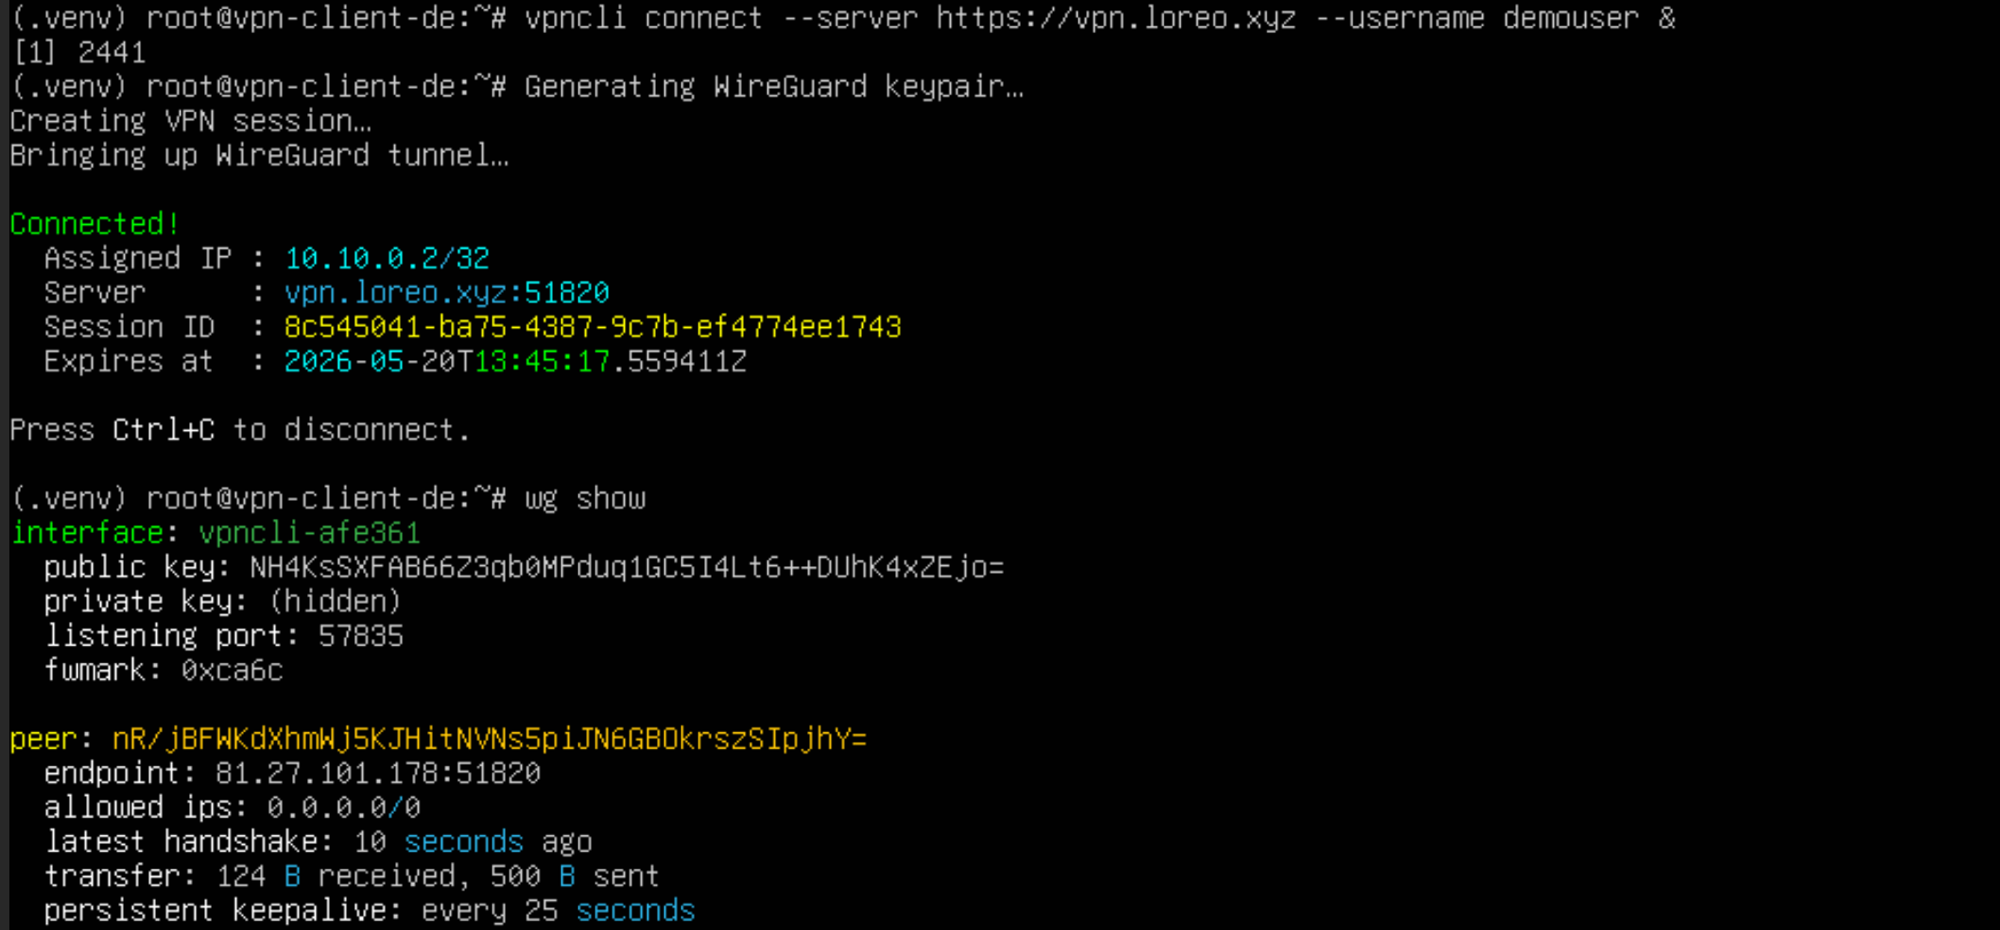
\includegraphics[width=\linewidth,height=0.32\textheight,
                       keepaspectratio]{func-07}\\[0.12em]
      {\tiny\ttfamily wg show} {\tiny--- тунель активний}
    \end{column}
    \begin{column}{0.32\textwidth}
      \centering
      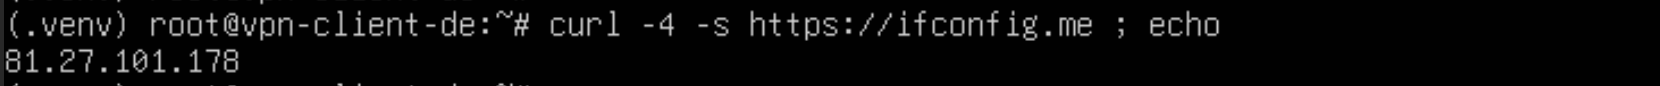
\includegraphics[width=\linewidth,height=0.26\textheight,
                       keepaspectratio]{func-08}\\[0.08em]
      {\tiny\ttfamily curl ifconfig.me} {\tiny з тунелем}\\[0.3em]
      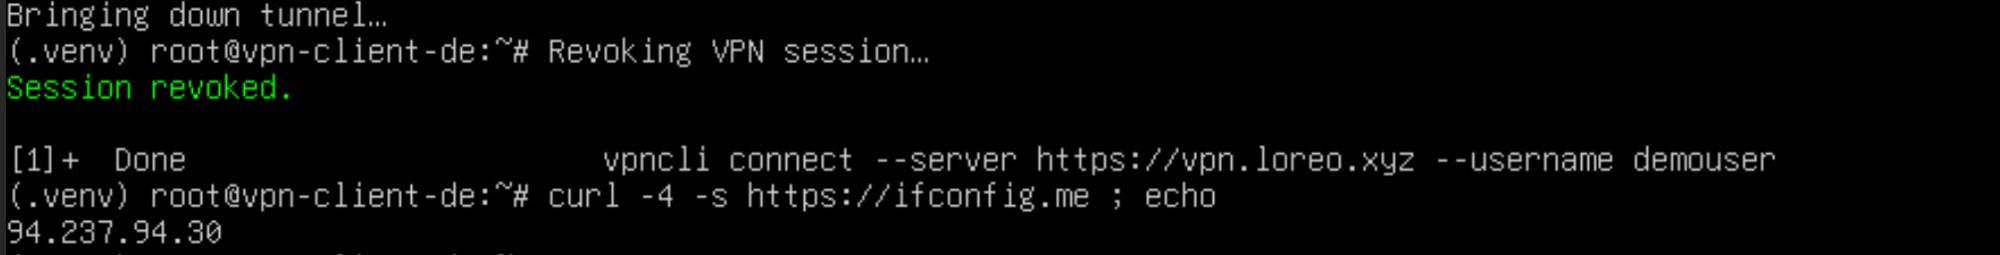
\includegraphics[width=\linewidth,height=0.26\textheight,
                       keepaspectratio]{func-09}\\[0.08em]
      {\tiny без тунелю}
    \end{column}
    \begin{column}{0.32\textwidth}
      \centering
      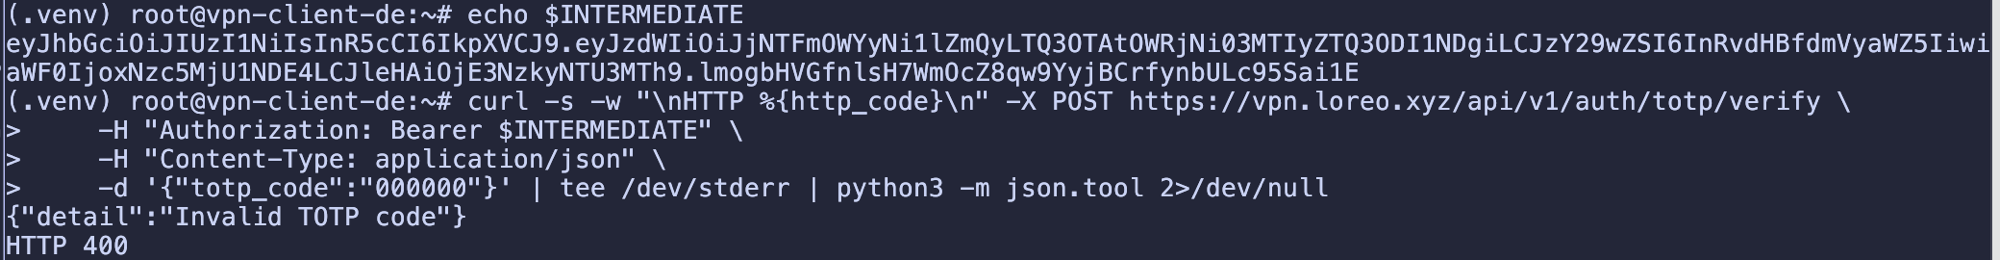
\includegraphics[width=\linewidth,height=0.20\textheight,
                       keepaspectratio]{func-12}\\[0.05em]
      {\tiny 400 --- невірний TOTP}\\[0.2em]
      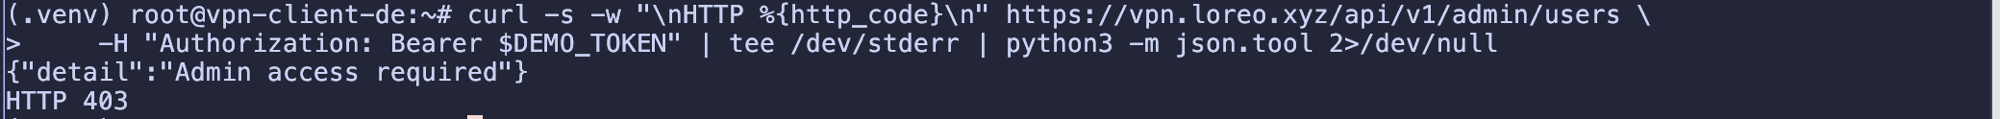
\includegraphics[width=\linewidth,height=0.20\textheight,
                       keepaspectratio]{func-13}\\[0.05em]
      {\tiny 403 --- не-адмін}\\[0.2em]
      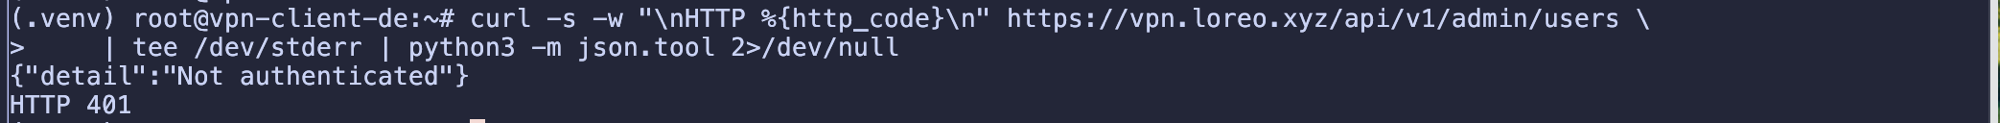
\includegraphics[width=\linewidth,height=0.20\textheight,
                       keepaspectratio]{func-14}\\[0.05em]
      {\tiny 401 --- без токена}
    \end{column}
  \end{columns}
\end{frame}

%% ── R6: CPU-таблиця ──────────────────────────────────────────────────────────
\begin{frame}
  \frametitle{CPU (резерв)}
  \centering
  \vspace*{0.7em}
  {\small
  \tstretch{1.5}
  \begin{tabularx}{\textwidth}{@{}Xrr@{}}
    \toprule
    \textbf{Конфігурація}
      & \textbf{\%soft (CPU)}
      & \textbf{На Мбіт/с} \\
    \midrule
    Наша система (Docker veth) & 34{,}80\;\% & 0{,}040\;\% \\
    WireGuard plain (Docker veth) & 20{,}56\;\% & 0{,}023\;\% \\
    \bottomrule
  \end{tabularx}
  \par\vspace{0.4em}
  {\footnotesize\color{clGrey}
    Різниця — Docker namespace (veth + netfilter), \textbf{не} від шифрування;
    той самий \texttt{wireguard.ko}.}
  }
\end{frame}

%% ── R7: Репозиторій (URL + QR) — LAST appendix frame ─────────────────────────
%% Answers «де знайти код?»
%% URL wrapped in \resizebox so the full string is always visible (never clipped).
\begin{frame}[c]
  \frametitle{Репозиторій (резерв)}
  \centering
  \vspace*{0.6em}
  {\normalsize\color{clGrey} Відкритий код (self-hosted):}\\[0.7em]
  \resizebox{0.9\textwidth}{!}{%
    \bfseries\color{clAccent}%
    \href{https://github.com/andriivaliukh/diploma}{%
      \texttt{github.com/andriivaliukh/diploma}}}%
  \par\vspace{1.0em}
  \qrcode[height=2.5cm]{https://github.com/andriivaliukh/diploma}
\end{frame}

\end{document}
